\subsection{FMI 2.0 Co-Simulation Wrapper}
\label{sec:impl_fmu}

The \texttt{FMUComponent} wrapper maps \ac{FMI}~2.0 Co-Simulation \acp{FMU} to the \texttt{CoSimComponent} interface of Section~\ref{sec:impl_component_interface}.
It realizes \ref{req:SR-05-01} under \ref{req:UR-05}.
The wrapper delegates \ac{FMI} calls to \texttt{fmpy}~\cite{dassault_systemes__catia-systems_fmpy_2026}.
It derives ports, parameters, value references, and direct-feedthrough metadata from the model description of the \ac{FMU}.

As described in Section~\ref{sec:237_cosim_fmi}, a Co-Simulation \ac{FMU} advances its model with an internal solver.
The \texttt{FMUComponent} class exposes this solver-owned simulation unit through the \syssimx{} component contract.
The resulting component can be connected, initialized, stepped, and inspected like any other \texttt{CoSimComponent}.

%%%%%%%%%%%%%%%%%%%%%%%%%%%%%%%%%%%%%%%%%%%%%%%%%%%%%%
\subsubsection{Architecture and Interface Mapping}

Figure~\ref{fig:impl_fmu_class} shows how the \ac{FMU} wrapper connects the framework contract to the \ac{FMI} runtime object.
The \texttt{FMUComponent} class inherits the template methods and port machinery from \texttt{CoSimComponent}.
It stores the \texttt{FMU2Slave} instance provided by \texttt{fmpy} as the backend object that executes \ac{FMI} calls.

\begin{figure}[t]
  \centering
  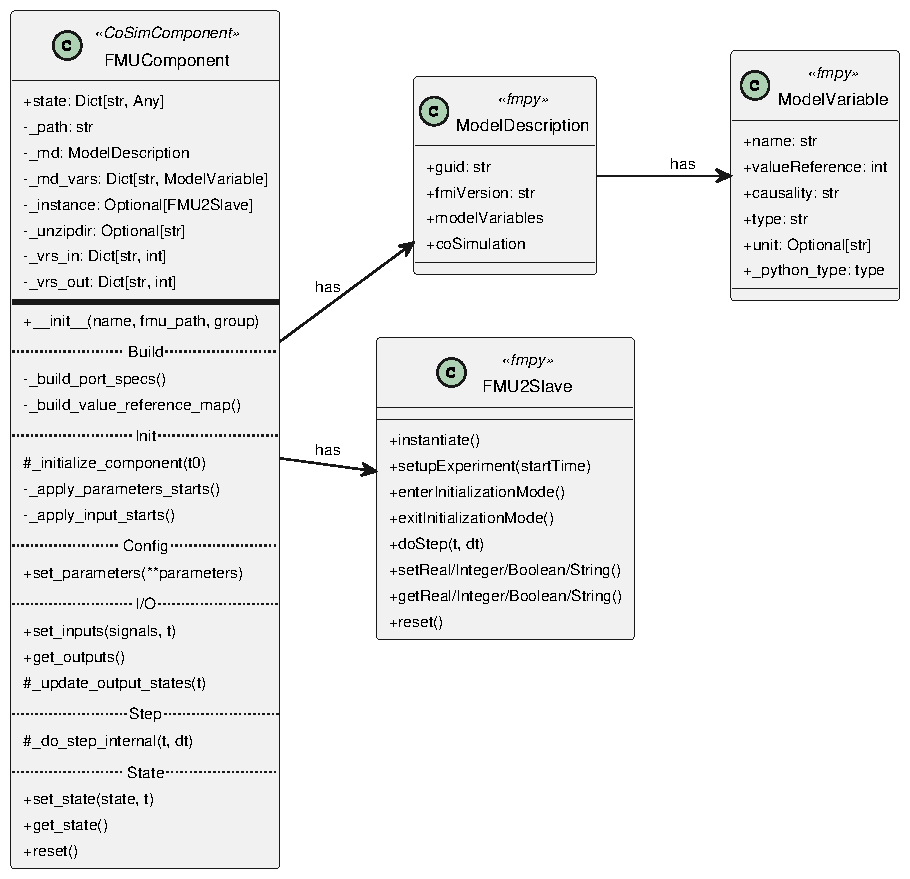
\includegraphics[width=\linewidth]{diagrams/out/pdf/class/components/FMUComponent.pdf}
  \caption[Class diagram of the \ac{FMU} wrapper]{Class diagram of the \ac{FMU} wrapper.
  The \texttt{FMUComponent} class adapts an \ac{FMI}~2.0 Co-Simulation \ac{FMU} to the \texttt{CoSimComponent} contract.
  The parsed model description supplies ports, parameters, value references, and direct-feedthrough metadata.
  The \texttt{FMU2Slave} instance executes the \ac{FMI} runtime operations.}
  \label{fig:impl_fmu_class}
\end{figure}

During construction, the wrapper parses the \ac{FMU} model description once.
It uses this metadata to create the \syssimx{}-level component interface.
Table~\ref{tab:fmu_mapping} lists the correspondence between \ac{FMI} artefacts and the component abstractions of Sections~\ref{sec:impl_port_system} and~\ref{sec:impl_component_interface}.

\begin{table}[t]
  \centering
  \small
  \caption[Mapping from \ac{FMI} model-description artefacts to \syssimx{} abstractions]{Mapping from \ac{FMI}~2.0 model-description artefacts to \syssimx{} component abstractions.
  The \texttt{FMUComponent} class computes this mapping once during construction.}
  \label{tab:fmu_mapping}
  \begin{tabular}{@{}p{0.42\linewidth}p{0.54\linewidth}@{}}
    \toprule
    \textbf{\ac{FMI} artefact} & \textbf{\syssimx{} abstraction} \\
    \midrule
    \texttt{ScalarVariable} with causality \texttt{input} or \texttt{output}
      & \texttt{PortSpec} with matching direction, data type, unit, and description \\
    \addlinespace
    \texttt{ScalarVariable} with causality \texttt{parameter}, \texttt{calculatedParameter}, or \texttt{structuralParameter}
      & Entry in the component's \texttt{parameters} dictionary with converted start value \\
    \addlinespace
    \texttt{ModelStructure/Outputs} dependencies
      & Entries in the \texttt{direct\_feedthrough} dictionary \\
    \addlinespace
    \texttt{valueReference}
      & Cached input and output reference maps grouped by \ac{FMI} base type \\
    \addlinespace
    \ac{FMI} unit strings such as \texttt{"m.s-2"}
      & Pint-compatible units on \texttt{REAL} ports after unit-string normalization \\
    \bottomrule
  \end{tabular}
\end{table}

The value-reference maps are cached once during construction.
\ac{FMI} variables are accessed by integer value references rather than by name.
The cached references are used for batched input writes and output reads grouped by \ac{FMI} base type.
This keeps runtime access independent of repeated name lookups.

Generic components use perturbation-based feedthrough detection, as described in Section~\ref{sec:impl_component_interface}.
\acp{FMU} can declare output dependencies in the \texttt{ModelStructure} element of the model description.
The \texttt{FMUComponent} class reads these dependencies directly and stores them in the feedthrough metadata.
This avoids additional \ac{FMI} calls and uses the dependencies declared by the \ac{FMU} exporter.

%%%%%%%%%%%%%%%%%%%%%%%%%%%%%%%%%%%%%%%%%%%%%%%%%%%%%%
\subsubsection{Lifecycle Realization}

The \texttt{FMUComponent} class realizes the primitive operations of the \texttt{CoSimComponent} base class through \ac{FMI}~2.0 calls.
During initialization, the wrapper extracts the \ac{FMU} archive and instantiates the \texttt{FMU2Slave}.
It calls \texttt{setupExperiment()}, enters initialization mode, applies parameters and input start values, and exits initialization mode.
The base-class template then publishes the initial outputs and records them in the component history.

A macro step is delegated to the \ac{FMI} \texttt{doStep()} call.
The call receives the current communication point $t$ and the communication step size $\Delta t$.
The base class handles time bookkeeping, output refresh, and history recording around this backend call.
Output refresh uses the cached value references.
The wrapper reads \ac{FMU} outputs through one getter call per active \ac{FMI} base type.
For \texttt{REAL} outputs, the declared unit is attached before the value is written to the corresponding \texttt{PortState}.

The hook \texttt{evaluate\_outputs(inputs, t)} supports algebraic-loop resolution.
It applies trial inputs and evaluates the \ac{FMU} outputs without committing a macro step.
The hook is used only for \acp{FMU} that support such zero-step evaluation.
It provides the instantaneous output values required by Section~\ref{sec:impl_algebraic_loops}.


%%%%%%%%%%%%%%%%%%%%%%%%%%%%%%%%%%%%%%%%%%%%%%%%%%%%%%
\subsubsection{State Access and Rollback Boundary}

The \texttt{FMUComponent} class implements the \texttt{get\_state()} and \texttt{set\_state()} methods as part of the framework state-transfer interface.
These methods are distinct from native \ac{FMI} state operations such as \texttt{getFMUState()} and \texttt{setFMUState()}.
The \texttt{get\_state()} method returns non-\texttt{fixed} and non-\texttt{local} \ac{FMU} variables with their current values and declared units.
The \texttt{set\_state()} method uses this dictionary to re-enter initialization, restore serialized values, and refresh the exposed output ports.

This dictionary state is intended for inspection, state transfer, and re-initialization.
Rollback for hybrid event localization requires an opaque snapshot of the internal \ac{FMU} solver state.
The generic \texttt{FMUComponent} only exposes the dictionary state and therefore leaves rollback to specialized subclasses.
Such subclasses can implement rollback when the concrete \ac{FMU} and solver provide a consistent restore mechanism.

%%%%%%%%%%%%%%%%%%%%%%%%%%%%%%%%%%%%%%%%%%%%%%%%%%%%%%
\subsubsection{Verification}

The verification targets the mapping from \ac{FMI} artefacts to the \texttt{CoSimComponent} contract.
The test subject is a purpose-built \ac{FMU} with two real inputs, two real outputs, one boolean parameter, and a declared feedthrough dependency.
Table~\ref{tab:fmu_verification} summarizes the checked properties.

\begin{table}[t]
  \centering
  \small
  \caption[\ac{FMI}-to-component mapping checks]{\ac{FMI}-to-component mapping checks for the purpose-built test \ac{FMU}.}
  \label{tab:fmu_verification}
  \begin{tabular}{p{5.8cm} p{8.8cm}}
    \toprule
    \textbf{Verified property} & \textbf{Expected outcome} \\
    \midrule
    Supported \ac{FMU} type
      & \ac{FMI}~2.0 Co-Simulation \acp{FMU} are accepted, while unsupported \ac{FMI} versions and Model Exchange \acp{FMU} are rejected \\
    \addlinespace
    Interface derivation
      & Ports, parameters, normalized units, and value-reference maps match \texttt{modelDescription.xml} \\
    \addlinespace
    Direct-feedthrough metadata
      & Dependencies declared in \texttt{ModelStructure} are reproduced in \texttt{direct\_feedthrough} \\
    \addlinespace
    Initialization and stepping
      & Parameters and input start values are applied during initialization, and \texttt{do\_step()} advances the \ac{FMU} by one communication step \\
    \addlinespace
    Zero-step output evaluation
      & \texttt{evaluate\_outputs()} returns outputs for supplied interface inputs without committing a macro step \\
    \addlinespace
    Reset and reuse
      & The wrapper can be reset and initialized again for another run \\
    \bottomrule
  \end{tabular}
\end{table}

These properties confirm that the \texttt{FMUComponent} class maps \ac{FMI}~2.0 Co-Simulation \acp{FMU} to the common component contract.
End-to-end integration with control, musculoskeletal, and \ac{FEM} components is evaluated in the controlled-pendulum case study in Chapter~\ref{chap:case_study}.
